\section{Aplicación}
\begin{frame}{Aplicación}
\begin{columns}
\begin{column}{0.9\textwidth}

\begin{table}[h]
\tiny
\centering
\begin{tabular}{|l|l|l|l|}
\hline
Nombre & Tipo de dato & Medida & Descripción \\
\hline
Cemento (variable 1) & continuo & kg en una mezcla $m^3$  &  Cantidad de cemento \\&&&presente en la mezcla \\
Escoria de alto horno (variable 2) & continuo & kg en una mezcla $m^3$ & Producto resultante \\&&&de distintas fundiciones\\&&& Mejora las capacidades \\&&& hidráulicas. \\
Ceniza volante (variable 3) & continuo & kg en una mezcla $m^3$ & Sustitutivo cemento.\\
Agua (variable 4) & continuo & kg en una mezcla $m^3$ & Agua en la mezcla.\\
Superplastificante (variable 5) & continuo & kg en una mezcla $m^3$ & Mejora la resistencia\\
Agregado grueso (variable 6) & continuo & kg en una mezcla $m^3$ &  Abaratador de la mezcla\\
Agregado fino (variable 7) & continuo & kg en una mezcla $m^3$ & Abaratador de la mezcla \\
Edad & continuo & Día (1-365) & Tiempo desde mezcla. \\
Resistencia a la compresión & continuo & MPa & \\
\hline
\end{tabular}
\caption{Resumen de las variables estudiadas}
\label{tab:Resumen Variables}
\end{table}
El tamaño de la muestra es de 1030 observaciones. 
\end{column}
\end{columns}
\end{frame}

\begin{frame}{Aplicación}
\begin{columns}
\begin{column}{0.9\textwidth}
\textbf{Objetivos:}

\begin{itemize}
\item Detallar y analizar patrones de comportamiento en los cementos en base a las características descritas. 
\item Crear y analizar distintos modelos que permitan la predicción de la resistencia a la compresión. 
\end{itemize}
\end{column}
\end{columns}
\end{frame}

\begin{frame}{Aplicación}
\begin{columns}
\begin{column}{0.9\textwidth}
\begin{figure}[h]
  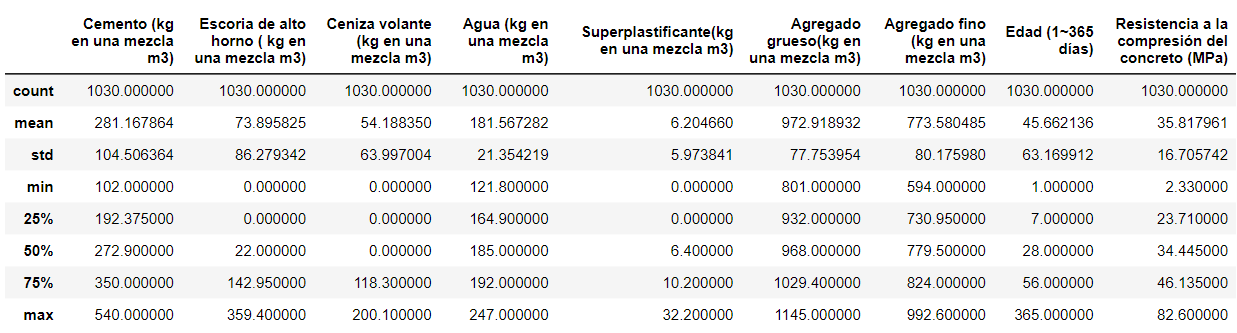
\includegraphics[scale=0.3]{Documentos Extra/Imagenes/Resumen_Basicos.png}
  \caption{Análisis descriptivo de los datos}
  \label{fig:resumen_basicos}
\end{figure}
\end{column}
\end{columns}
\end{frame}

\begin{frame}{Aplicación}
\begin{columns}
\begin{column}{0.9\textwidth}
\textbf{Analisis de componentes principales:}
\begin{figure}[h]
  \centering
  \includegraphics[scale=0.3]{Documentos Extra/Imagenes/Gráfico_varianza_explicada.png}
  \caption{Proporción de varianza acumulada explicada por las componentes principales.}
  \label{fig:varianza acumulada}
\end{figure}

En particular la varianza explicada por cada una de las componentes:
\begin{equation}
(0.25 \enspace 0.22 \enspace 0.16 \enspace 0.12 \enspace 0.11 \enspace 0.09 \enspace 0.03 \enspace 0.02 \enspace 0.  )
\end{equation}
\end{column}
\end{columns}
\end{frame}

\begin{frame}{Aplicación}
\begin{columns}
\begin{column}{0.9\textwidth}
Las componentes principales tienen las cargas:
\begin{align}
Z_1&=(0,04;0.16;-0.37  ; 0.56  ;   -0.54  ;  0.06 ;  -0.38  ; 0.26  ; -0.11)\mathbf{x}^T\\
Z_2&=(0.54 ; 0.14 ;  -0.27  ; -0.12 ;   0.25  ; -0.22 ;  -0.19 ;  0.25  ;  0.63)\mathbf{x}^T\\
Z_3&=(0.36 ; -0.7 ;  0.02 ;-0.12; -0.19  ; 0.55 ; 0 ;   0.17 ; 0.03)\mathbf{x}^T
\end{align}
\end{column}
\end{columns}
\end{frame}

\begin{frame}{Aplicación}
\begin{columns}
\begin{column}{0.9\textwidth}
Modelo lineal de regresión:
\begin{equation}
\begin{split}
Y=&-51.45+0.13 X_1+0.11X_2+0.1X_3-0.12X_4+0.26X_5\\&+  0.03X_6+0.03X_7+0.11X_8
\end{split}
\end{equation}
Resultados: 
\begin{itemize}
\item Conjunto de entrenamiento
\begin{itemize}
\item \textbf{MSE: }$108,35$
\item $R^2: 0.61$
\end{itemize}
\item Conjunto de prueba
\begin{itemize}
\item \textbf{MSE: }$106,02$
\item $R^2:0.61$
\end{itemize}
\end{itemize}
\end{column}
\end{columns}
\end{frame}

\begin{frame}{Aplicación}
\begin{columns}
\begin{column}{0.9\textwidth}
\begin{figure}[h]
  \centering
  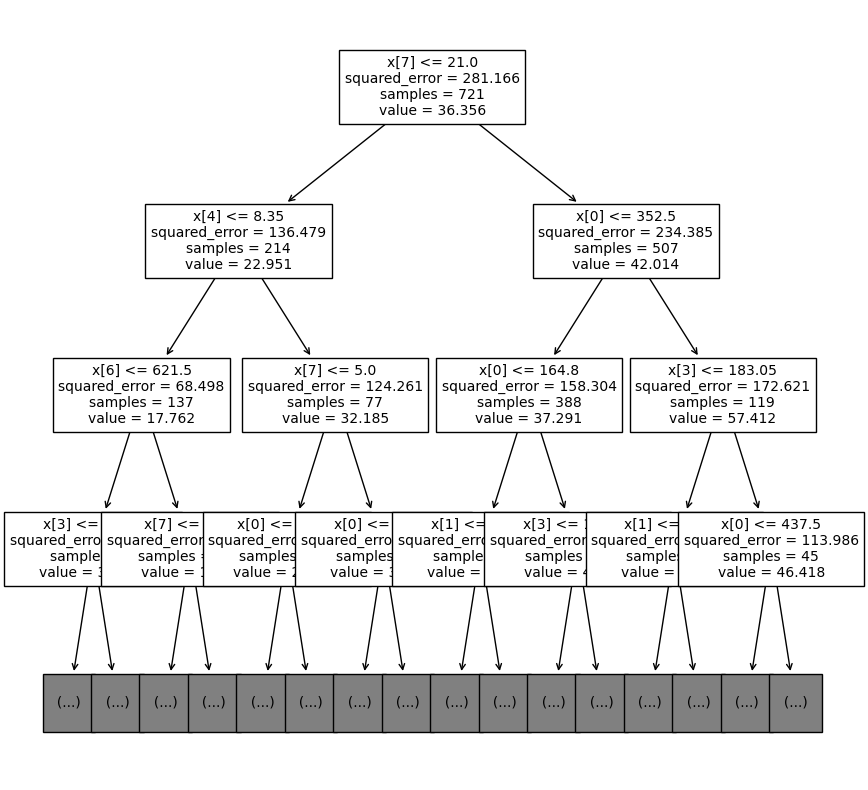
\includegraphics[scale=0.33]{Documentos Extra/Imagenes/Arbol.png}
  \caption{Diagrama resultante hasta profundidad 3}
  \label{fig:diagrama arbol}
\end{figure}
  
\end{column}
\end{columns}
\end{frame}

\begin{frame}{Aplicación}
\begin{columns}
\begin{column}{0.9\textwidth}
\textbf{Árbol de regresión: }

\begin{itemize}
\item Conjunto de entrenamiento
\begin{itemize}
\item \textbf{MSE: }$1,15$
\item $R^2: 0,996$
\end{itemize}
\item Conjunto de prueba
\begin{itemize}
\item \textbf{MSE: }$53,28$
\item $R^2: 0,803$
\end{itemize}
\end{itemize}

\emph{Observación: }las medidas del conjunto de prueba nos dice que estamos ante un caso en el que se ha producido un sobreajuste. 
\end{column}
\end{columns}
\end{frame}

\begin{frame}{Aplicación}
\begin{columns}
\begin{column}{0.9\textwidth}
\begin{figure}[h]
  \centering
  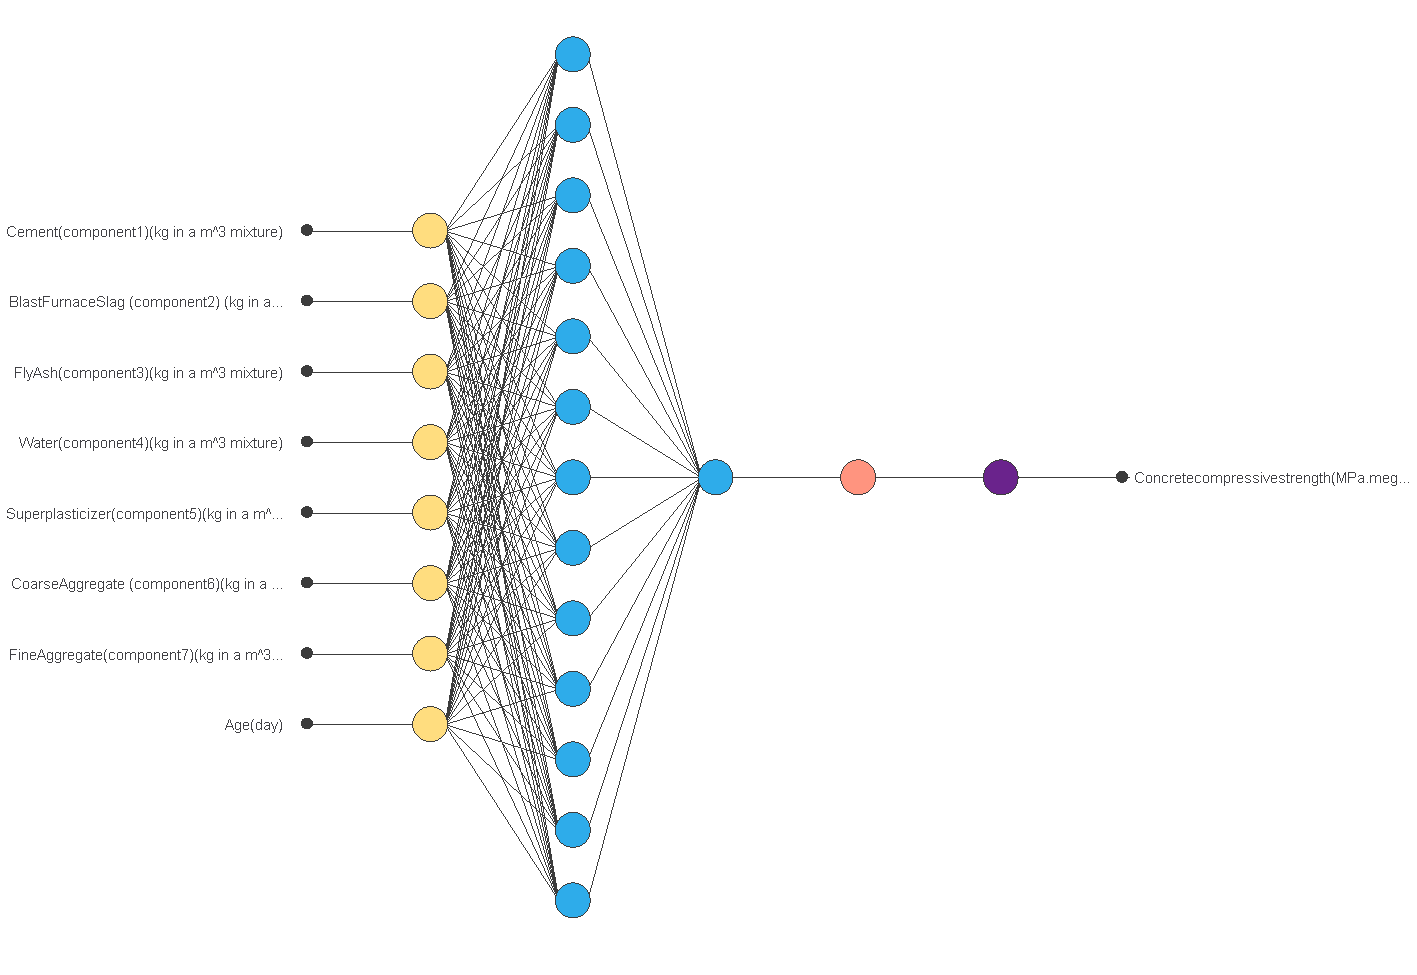
\includegraphics[scale=0.25]{Documentos Extra/Imagenes/concrete archiquecture.png}
  \caption{Estructura de la red neuronal, realizada con el programa Neural Designer.}
  \label{fig:estructura red neuronal}
\end{figure}
  
\end{column}
\end{columns}
\end{frame}

\begin{frame}{Aplicación}
\begin{columns}
\begin{column}{0.9\textwidth}
\textbf{Red neuronal:}

\begin{itemize}
\item Conjunto de entrenamiento
\begin{itemize}
\item \textbf{MSE: }$45,748$
\item $R^2: 0,837$
\end{itemize}
\item Conjunto de prueba
\begin{itemize}
\item \textbf{MSE: }$51,805$
\item $R^2: 0,809$
\end{itemize}
\end{itemize}

\emph{Observación:} los resultados obtenidos con el software Neural Designer son mejores. 
\end{column}
\end{columns}
\end{frame}


\begin{frame}{Aplicación}
\begin{columns}
\begin{column}{0.9\textwidth}
\textbf{Comparación modelos:}
\begin{figure}[h]
 \centering
  \subfloat[Regresión Lineal]{
   \label{fig:regresion_lineal}
    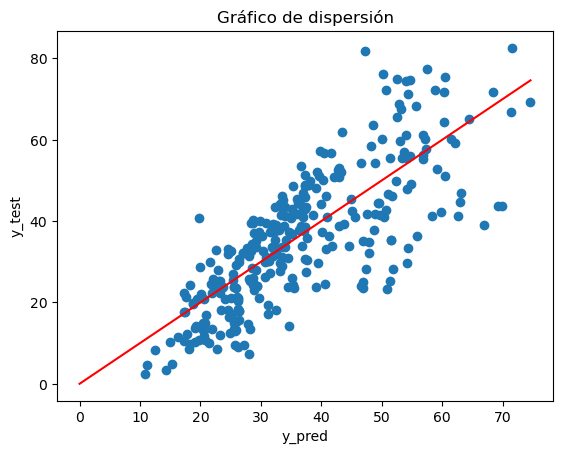
\includegraphics[width=0.3\textwidth]{Documentos Extra/Imagenes/Datos PruebasRegresionLineal.png}}
  \subfloat[Árbol de regresión]{
   \label{fig:regression_tree}
    \includegraphics[width=0.3\textwidth]{Documentos Extra/Imagenes/Datos PruebasÁrbolesRegresion.png}}
    \subfloat[Red neuronal]{
   \label{fig:red_neuronal}
    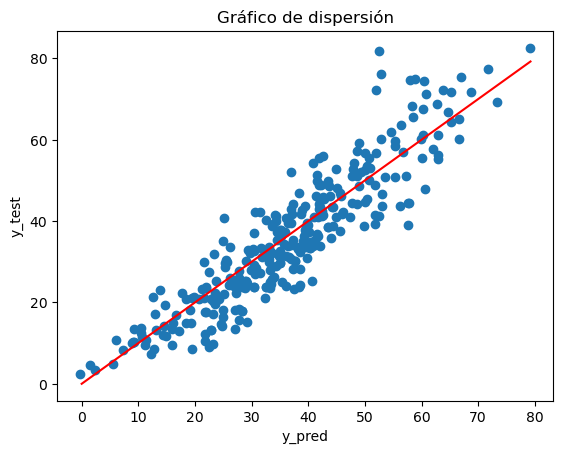
\includegraphics[width=0.3\textwidth]{Documentos Extra/Imagenes/Datos PruebasRedNeuronal.png}}
 \caption{Gráficos de comparación de los valores predichos con el valor real.}
  \label{fig: comparación}
\end{figure}


\end{column}
\end{columns}
\end{frame}